\documentclass{exam}
\usepackage[utf8]{inputenc}
\usepackage{lmodern}
\usepackage{microtype}

% \usepackage[parfill]{parskip}
\usepackage[dvipsnames]{xcolor}
\usepackage{amsmath}
\usepackage{amsfonts}
\usepackage{amsthm}
\usepackage{siunitx}
\DeclareSIUnit\year{yr}
\DeclareSIUnit\foot{ft}
\DeclareSIUnit\litre{\liter}

\usepackage{skull}

\usepackage{pgfplots}
\usepgfplotslibrary{polar}
\pgfplotsset{compat=1.11}
\usepgfplotslibrary{statistics}
\usepackage{graphicx}
\usepackage{sidecap}
\sidecaptionvpos{figure}{c}
\usepackage{float}
\usepackage{gensymb}
\usepackage{tkz-euclide}
\usetkzobj{all}
\usepackage{commath}
\usepackage{hyperref}
\usepackage{enumitem}
\usepackage{wasysym}
\usepackage{multicol}
\usepackage{mathtools}
\usepackage{tcolorbox}
\usepackage{tabularx}
\usepackage[version=4]{mhchem}
\usepackage{changepage}
\usepackage{listings}
\lstset{basicstyle=\ttfamily\linespread{0.8}\small}

\renewcommand*{\thefootnote}{\fnsymbol{footnote}}

\newtheorem*{thm}{Theorem}
\newtheorem*{iden}{Identity}
\newtheorem*{lemma}{Lemma}
\newtheorem{obs}{Observation}
\theoremstyle{definition}
\newtheorem*{defn}{Definition}
\newtheorem*{ex}{Example}
\newtheorem{con}{Construction}
\newtheorem*{alg}{Algorithm}

\newtheoremstyle{break}
  {\topsep}{\topsep}%
  {\itshape}{}%
  {\bfseries}{}%
  {\newline}{}%
\theoremstyle{break}
\newtheorem*{bthm}{Theorem}

% russian integral
\usepackage{scalerel}
\DeclareMathOperator*{\rint}{\scalerel*{\rotatebox{17}{$\!\int\!$}}{\int}}

% \DeclareMathOperator*{\rint}{\int}

\pgfplotsset{vasymptote/.style={
    before end axis/.append code={
        \draw[densely dashed] ({rel axis cs:0,0} -| {axis cs:#1,0})
        -- ({rel axis cs:0,1} -| {axis cs:#1,0});
    }
}}

% \pointsinrightmargin
\boxedpoints
\pointname{}

\newcommand{\questioA}{\question[\texttt{\textbf{\color{Cerulean} A}}]}
\newcommand{\questioM}{\question[\texttt{\textbf{\color{PineGreen} M}}]}
\newcommand{\questioE}{\question[\texttt{\textbf{\color{WildStrawberry} E}}]}
\newcommand{\questioS}{\question[\texttt{\textbf{\color{Goldenrod} S}}]}
\newcommand{\questioO}{\question[\texttt{\textbf{\color{BurntOrange} O}}]}

\newcommand{\parA}{\part[\texttt{\textbf{\color{Cerulean} A}}]}
\newcommand{\parM}{\part[\texttt{\textbf{\color{PineGreen} M}}]}
\newcommand{\parE}{\part[\texttt{\textbf{\color{WildStrawberry} E}}]}
\newcommand{\parS}{\part[\texttt{\textbf{\color{Goldenrod} S}}]}
\newcommand{\parO}{\part[\texttt{\textbf{\color{BurntOrange} O}}]}

\newcommand{\subparA}{\subpart[\texttt{\textbf{\color{Cerulean} A}}]}
\newcommand{\subparM}{\subpart[\texttt{\textbf{\color{PineGreen} M}}]}
\newcommand{\subparE}{\subpart[\texttt{\textbf{\color{WildStrawberry} E}}]}
\newcommand{\subparS}{\subpart[\texttt{\textbf{\color{Goldenrod} S}}]}
\newcommand{\subparO}{\subpart[\texttt{\textbf{\color{BurntOrange} O}}]}

\newcommand{\mainHeader}[2]{\section*{NCEA Level 2 Mathematics\\#1. #2}}
\newcommand{\mainHeaderHw}[2]{\section*{NCEA Level 2 Mathematics (Homework)\\#1. #2}}
\newcommand{\seealso}[1]{\begin{center}\emph{See also #1.}\end{center}}
\newcommand{\drills}[1]{\begin{center}\emph{Drill problems: #1.}\end{center}}
\newcommand{\basedon}[1]{\begin{center}\emph{Notes largely based on #1.}\end{center}}


\begin{document}

\mainHeader{17}{Number Sequences and Fractals}
A number sequence is an arrangement of numbers in which each successive number follows the last according to
a uniform rule. More precisely, a number sequence is a correspondence between the counting numbers and a set
of numbers: $ (a_n) = a_1, a_2, a_3, \dots $.

\subsection*{Arithmetic Sequences}
Arithmetic sequences are the simplest kind of interesting sequence.
\begin{defn}
  An arithmetic sequence is a number sequence in which each successive term may be found by adding the
  same number; formally, a sequence is arithmetic if $ a_{n + 1} = a_n + k $ for every $ n > 1 $ and for
  some constant $ k $.
\end{defn}
\begin{ex}
  In the following sequence, $ a_1 = 2 $ and $ a_{n + 1} = a_n + 3 $.
  \begin{displaymath}
    2, 5, 8, 14, 17, \cdots
  \end{displaymath}
\end{ex}

For arithmetic sequences, if we know the initial value and the constant difference then we can find each number
in the sequence easily.

\begin{thm}
  If $ a_1, a_2, \cdots $ is an arithmetic sequence with constant difference $ k $, then $ a_n = a_1 + (n - 1)k $.
  (This is called the \emph{general term} of the sequence.)
\end{thm}
\begin{proof}
  $ a_n = a_{(n - 1)} + k = a_{(n - 2)} + 2k = \cdots = a_{(n - (n - 1))} + (n - 1)k $.
\end{proof}

Suppose we want to find the \emph{sum} of the first $ n $ values of some sequence $ a_1, a_2, \dots $. For a simple
example, we turn to a problem from last week.
\begin{ex}
  We will find the sum of the first $ n $ counting numbers. Behold:
  \begin{displaymath}
    \begin{array}{ccccccccccccccccc}
    1 &+& 2 &+& 3 &+& 4 &+& \cdots &+& (n - 3) &+& (n - 2) &+& (n - 1) &+& n\\
    n &+& (n - 1) &+& (n - 2) &+& (n - 3) &+& \cdots &+& 4 &+& 3 &+& 2 &+& 1
    \end{array}
  \end{displaymath}

  Adding the two rows together and dividing by two, we obtain the result that
  \begin{displaymath}
    1 + \cdots + n = \frac{n(n + 1)}{2}.
  \end{displaymath}

  (This is called the $ n$th partial sum of the series $ 1 + 2 + 3 + \cdots + n $.)
\end{ex}

We now turn our attention to finding the $ n$th partial sum of the series $ a_1 + a_2 + a_3 + \cdots + a_n $. By the
theorem above, we can rewrite this as
\begin{align*}
  a_1 + a_2 + a_3 + \cdots + a_n &= [a_1 + (1 - 1)k] + [a_1 + (2 - 1)k] + [a_1 + (3 - 1)k] + \cdots + [a_1 + (n - 1)k]\\
                                 &= [a_1 + \cdots + a_1] + [0k + 1k + 2k + \cdots + (n-1)k]\\
                                 &= na_1 + k[0 + 1 + 2 + \cdots + (n - 1)]\\
                                 &= na_1 + k \frac{n(n - 1)}{2}.
\end{align*}

Hence, we have proved the following
\begin{thm}
  The $ n$th partial sum of the series $ a_1 + a_2 + a_3 + \cdots + a_n $ is given by
  \begin{displaymath}
    na_1 + k \frac{n(n - 1)}{2}
  \end{displaymath}
\end{thm}
(but you should memorise the idea of the proof, not the formula.)

\subsection*{Geometric Sequences}
The next simplest kind of sequence after arithmetic sequences (where you add a constant term) is a geometric
sequence (where you multiply by a constant term).
\begin{defn}
  A geometric sequence is a number sequence in which each successive term may be found by multiplying by the
  same number; formally, a sequence is geometric if $ a_{n + 1} = ka_n $ for every $ n > 1 $ and for
  some constant $ k $.
\end{defn}

\begin{ex}\leavevmode
  \begin{enumerate}
    \item $ a_1 = 1 $, $ a_n = 2a_{n - 1} $: $ 1, 2, 4, 6, 8, ... $ (the binary sequence).
    \item $ a_1 = 100 $, $ a_n = \frac{1}{10} a_{n - 1} $: $ 100, 10, 1, 0.1, 0.01, ... $.
    \item $ a_1 = 1 $, $ a_n = -1 a_{n - 1} $: $ 1, -1, 1, -1, ... $.
  \end{enumerate}
\end{ex}


\begin{thm}
  If $ a_1, a_2, \cdots $ is an geometric sequence with constant ratio $ k $, then:
  \begin{enumerate}
    \item the general term of the sequence is $ a_n = a_1 k^{n - 1} $.
    \item the $ n$th partial sum of the sequence is $ s_n = a_1 \frac{1 - k^n}{1 - k}$.
  \end{enumerate}
\end{thm}
\begin{proof}\leavevmode
  \begin{enumerate}
    \item Exercise.
    \item This proof uses a little trick:
      \begin{align*}
               s_n &= a_1 k^0 + a_1 k^1 + a_1 k^2 + \cdots + a_1 k^{n - 1} = a_1^n (1 + k + k^2 + \cdots + k^{n - 1})\\
        (1 - k)s_n &= a_1 (1-k)(1 + k + k^2 + \cdots + k^{n - 1})\\
                   &= a_1 [(1 + k + k^2 + \cdots + k^{n - 1}) - k(1 + k + k^2 + \cdots + k^{n - 1})]\\
                   &= a_1 [(1 + k + k^2 + \cdots + k^{n - 1}) - (k + k^2 + k^3 + \cdots + k^n)]\\
                   &= a_1 [1 - k^n]\\
               s_n &= a_1 \frac{1 - k^n}{1 - k}.
      \end{align*}
  \end{enumerate}
\end{proof}

Geometric sequences are slightly more interesting than arithmetic sequences; if we add up all the terms of an arithmetic sequence, the
resulting partial sums always grow towards $ \pm\infty $. On the other hand, it is possible for the sum of all the terms of a
geometric sequence to tend to some finite value. One case in which this happens is the following example.
\begin{ex}
  Consider the geometric sequence given by $ a_n = \frac{1}{2}^n $:
  \begin{displaymath}
    1, \frac{1}{2}, \frac{1}{4}, \frac{1}{8}, \frac{1}{16}, \dots
  \end{displaymath}

  The sum $ 1 + 1/2 + 1/4 + \cdots $ converges to 1, as shown graphically here.
  \begin{center}
    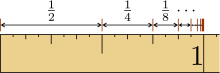
\includegraphics[width=0.3\textwidth]{geomconverge}
  \end{center}
\end{ex}
On the other hand, it is very easy for series to diverge (not tend towards any finite value): just take $ k > 1 $. More interestingly,
we can consider the following sequence:
\begin{ex}
  Consider the geometric sequence given by $ a_n = (-1)^n $:
  \begin{displaymath}
    1, -1, +1, -1, +1, \dots
  \end{displaymath}

  The sum $ 1 - 1 + 1 - 1 + \cdots $ does not converge as it jumps between $ +1 $ and $ -1 $ infinitely often.
\end{ex}

Let us try to work out under which conditions the geometric series \emph{does} converge. We want to look at
the behaviour of the quantity $ a_1 \frac{1 - k^n}{1 - k} $ as $ n $ grows. We make the following observations:
\begin{enumerate}
  \item If $ k = 1 $, then the quantity is undefined: but then, the sequence looks like $ a_1 + a_1 + \cdots $, which
        grows arbitrarily large and so the sum diverges.
  \item If $ k > 1 $, then the sum also grows arbitrarily large and the series diverges.
  \item If $ k = -1 $, then the sum diverges but now oscillates around zero instead of growing to infinity.
  \item If $ k < -1 $, then the sum grows arbitrarily large and oscillates between being positive and negative, so diverges.
  \item If $ -1 < k < 1 $, then $ k^n $ gets smaller as $ n $ increases --- so tends to zero, and the sum of the series
        as $ n \to \infty $ is given by $ \lim a_n = a_1 \frac{1}{1 - k} $.
\end{enumerate}

In summary, we have seen that:
\begin{itemize}
  \item The general term of an arithmetic sequence is $ a_n = a_1 + (n - 1)k $.
  \item The $ n$th partial sum of an arithmetic series is $ s_n =  na_1 + k \frac{n(n - 1)}{2} $.
  \item The general term of a geometric sequence is $ a_n = a_1 k^{n - 1} $.
  \item The $ n$th partial sum of a geometric series is $ s_n = a_1 \frac{1 - k^n}{1 - k}$.
  \item If $ -1 < k < 1 $ is the ratio of a geometric series, then the series converges to $ \lim a_n = a_1 \frac{1}{1 - k}$
\end{itemize}
These five facts are the important things to remember.

\clearpage
\subsection*{Fractals}
We now move from sequences of numbers to sequences of geometric objects, with an very brief overview of fractals. Informally,
a fractal is a geometric figure with the property of self-similarity: if you zoom in, it looks `the same'. Many examples of
fractal geometry can be found in nature; the traditional example is a coastline:
\begin{center}
  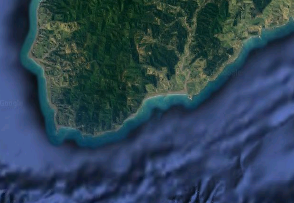
\includegraphics[height=0.15\textwidth]{coast1}
  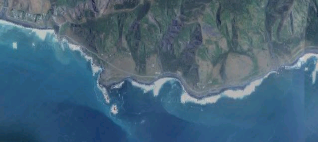
\includegraphics[height=0.15\textwidth]{coast2}
  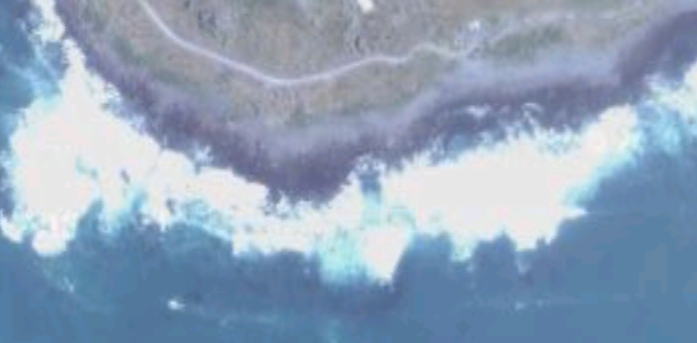
\includegraphics[height=0.15\textwidth]{coast3}
\end{center}
As we zoom in, the coastline reveals new `wiggles' that we couldn't see at a larger scale --- but it always looks wiggly in the same way, no
matter how far you zoom in.

\begin{con}[H-fractal]
  Begin at step one with a line segment of length 1. Then at each step $ n $, add a line segment of length $ \left(\frac{1}{\sqrt{2}}\right)^{n - 1} $ to
  the endpoints of each line segment created at step $ n - 1 $. (The lengths are purely aesthetic.)
\end{con}
The curve produced is the H-fractal; a Python script to draw it (\texttt{hcurve.py}) is given in the appendices. Below we have the curve after
the second, fourth, eighth, and twelfth steps.
\begin{center}
  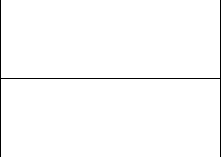
\includegraphics[width=0.4\textwidth]{hcurve2}\quad
%   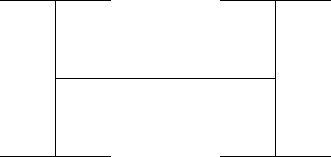
\includegraphics[width=0.25\textwidth]{hcurve3}
  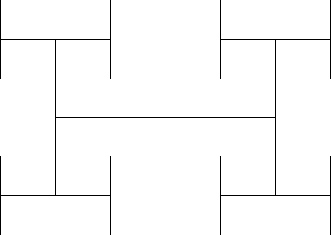
\includegraphics[width=0.4\textwidth]{hcurve4}\\
  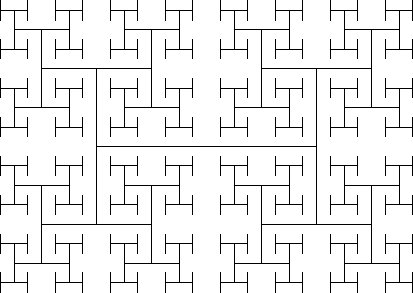
\includegraphics[width=0.4\textwidth]{hcurve8}\quad
  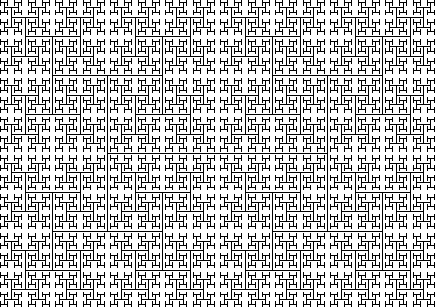
\includegraphics[width=0.4\textwidth]{hcurve12}
\end{center}

How many segments are present at the $ n$th step? At the first step we have one, at the second three, at the third seven, at the fourth fifteen,
and so on: the number seems to be $ 2^n - 1 $ segments. How do we prove this? Well, suppose we have $ k $ endpoints at the $ n - 1 $th step. Then
at the $ n$th step, we add $ k $ lines and hence $ 2k $ endpoints --- so the number of endpoints doubles each time. Initially we have two endpoints, so the number
of endpoints added at each step follows a geometric sequence with initial term 2 and ratio 2: at step $ n $, we add $ 2^n $ endpoints. The sum
of all these endpoints is simply $ 2 \frac{1 - 2^n}{1 - 2} = 2(2^n - 1) $ (using our formula for the partial sum of a geometric series); and
every line has two endpoints, so we must divide by two.

An interesting property of this curve is that, as well as having `infinite length', it is space-filling --- when we complete the construction
at infinity, the curve will cover every point in the rectangle that it is bounded by.\footnote{More precisely, we can pick some number $ N $ such that
after the $ N$th step, the curve comes within any distance $ \delta $ of any point within the rectangle that we want. Obviously if $ \delta $ is small
then we need $ N $ to be (very) large, but the point is that it's theoretically possible!}

Other methods of producing fractals involve removing portions of a figure rather than adding portions.

\begin{con}[Cantor set]
  At step 1, begin with a unit segment; then at step $ n $, remove the middle third of each of the segments remaining from
  the previous step.
\end{con}
This construction, pictured below, was first discovered by Henry John Stephen Smith in 1874 and entered mainstream mathematical knowledge
in 1883 due to Georg Cantor (the father of set theory). The Cantor set itself, produced by continuing the construction to infinity, still
has infinitely many points but has (in a precise sense) zero length. A Python script to draw it (\texttt{cantor.py}) is given in the appendices.
\begin{center}
  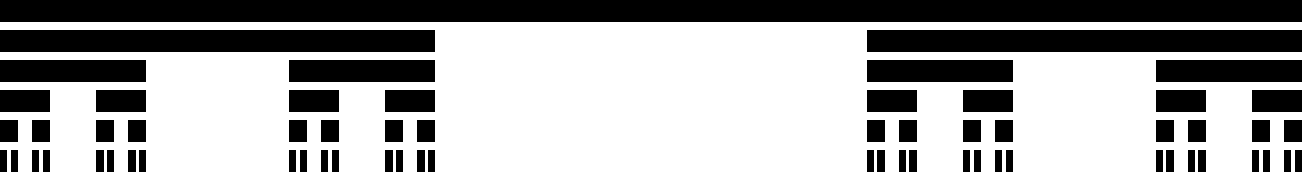
\includegraphics[width=\textwidth]{cantor}
\end{center}
Our initial length is 1; at each step we remove precisely $ 1/3 $ of the remaining length, or equivalently we keep $ 2/3 $ of the remaining
length; so the length of the set at step $ n $ is given by the geometric sequence with general term $ \left(\frac{2}{3}\right)^{n - 1} $. In
particular, since $ 2/3 $ is less than 1, if we take $ n \to \infty $ the sequence goes to zero.

\begin{con}[Sierpinski triangle]
  At step 1, we start with a filled equilateral triangle. At the $ n$th step, split each filled triangle into four equilateral triangles
  and remove the central triangle.
\end{con}
If this construction is carried on forever, the result is the Sierpinski triangle. This fractal was first described by a Polish mathematician,
Waclaw Sierpinski, in 1916, and is a generalisation of the Cantor construction to two dimensions. Similarly to the Cantor set, the measure of
the Sierpinski triangle (in this case the area) is zero but it still contains infinitely many points! A Python script to draw it (\texttt{sierp.py})
is given in the appendices; below, we have the triangle after two, three, four, and nine iterations.
\begin{center}
  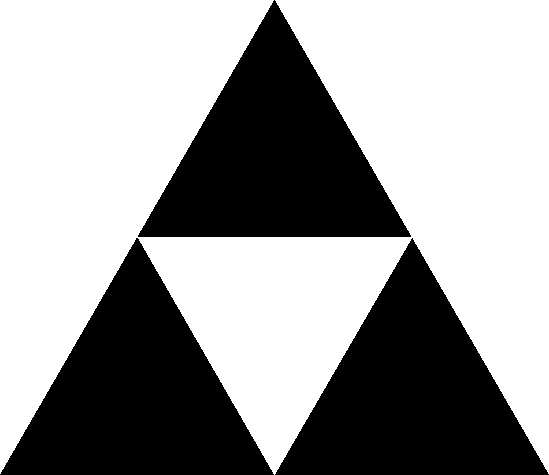
\includegraphics[width=0.2\textwidth]{sierp2}
  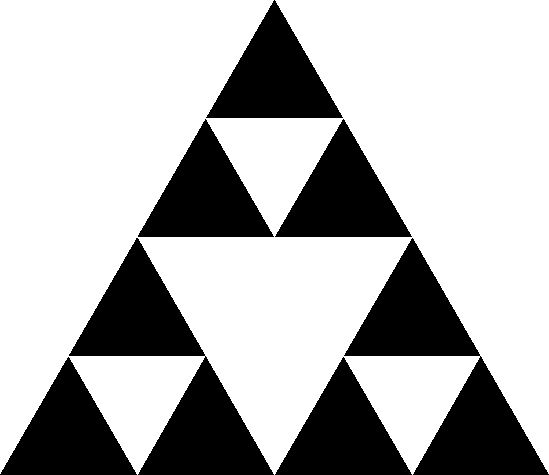
\includegraphics[width=0.2\textwidth]{sierp3}
  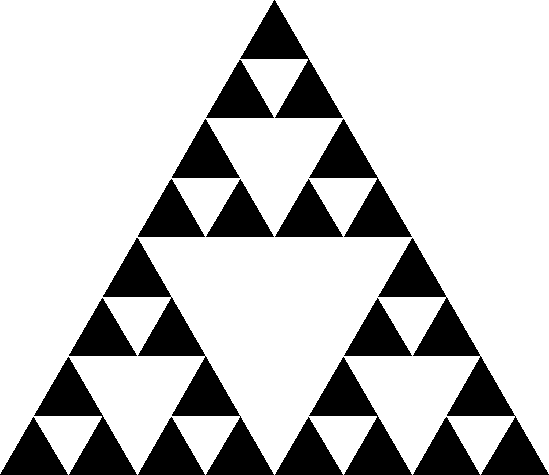
\includegraphics[width=0.2\textwidth]{sierp4}
  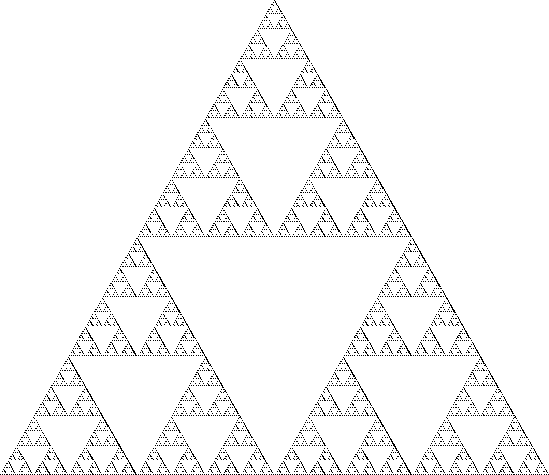
\includegraphics[width=0.2\textwidth]{sierp9}
\end{center}

One possible generalisation to three dimensions is the Sierpinski tetrahedron, produced by removing pyramids from a pyramid; two are pictured
below.\footnote{CC BY-SA 3.0, \url{https://commons.wikimedia.org/w/index.php?curid=647064}}
\begin{center}
  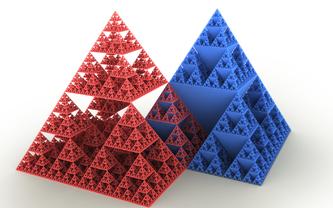
\includegraphics[width=0.4\textwidth]{sierpyramid}
\end{center}

\subsection*{Questions}
\begin{questions}
  \fullwidth{\subsubsection*{Sequences and Series}}
  \question The following are snippets of sequences that are either arithmetic or geometric. Give the general term of each. (In each case, $ a_1 = 1 $.)
    \begin{parts}
      \part $ \dots, \frac{1}{27}, \frac{1}{81}, \frac{1}{243}, \dots $
      \part $ \dots, 5, 7, 9, \dots $
      \part $ \dots, -10, 100, -1000, \dots $
      \part $ \dots, 0.02116, 0.0097336, 0.004477456, \dots $
    \end{parts}
  \question Prove that the general term of a geometric sequence $ (a_n) $ with constant ratio $ k $ is $ a_1 k^{n - 1} $.
  \question Compare the formulae that give the general term of an arithmetic sequence and a geometric sequence.
  \question The Fibonacci sequence is the sequence defined by $ f_1 = 1 $, $ f_2 = 1 $, and $ f_n = f_{n - 2} + f_{n - 1} $.
            The first few numbers in the sequence are $ 1, 1, 2, 3, 5, 8, 13, 21, \cdots $.
    \begin{parts}
      \part The Fibonacci sequence was studied by Leonardo of Pisa (Fibonacci) in the middle ages, in his book
            \emph{Liber Abaci} (``Book of Calculation''). In this book appeared the following problem:
            \begin{center}
              \itshape A pair of rabbits one month old are too young to produce more rabbits, but suppose that in their
              second month and every month thereafter they produce a new pair. If each new pair of rabbits does the same,
              and none of the rabbits die, how many pairs of rabbits will there be at the beginning of each month?
            \end{center}
            Show that the solution is given by the Fibonacci sequence.
      \part Prove that the Fibonacci sequence is neither an arithmetic nor a geometric sequence.
      \part It turns out that, despite not being a geometric sequence, the ratios of adjacent Fibonacci numbers tend to
            a constant value. Taking this to be true without proof, we will calculate what this ratio is.
        \begin{subparts}
          \subpart Justify why, if $ n $ is very large, $ \frac{f_{n + 1}}{f_n} \approx \frac{f_{n}}{f_{n - 1}} $.
          \subpart Show that, if $ x = \frac{f_n + 1}{f_n} $, then $ x \approx 1 + \frac{1}{x} $.
          \subpart Show that $ x = \frac{1}{2} + \frac{\sqrt{5}}{2} $. (This value is usually called $ \varphi $, the golden ratio.)
          \subpart Experimentally verify that this is the approximate ratio between adjacent values for the first few values of the Fibonacci series.
          \subpart Explain why we have \emph{not} proved that this is the eventual ratio between adjacent values of the Fibonacci sequence.
        \end{subparts}
    \end{parts}
  \question According to legend, the game of chess was invented by an ancient Indian minister for his ruler; the ruler was
            impressed, and asked the minister what reward he wanted, and the minister requested that the ruler take
            a chessboard and give him one grain of wheat on the first square, two grains on the second, four on the third,
            eight on the fourth, and so on. The ruler laughed it off as a meager prize for such a brilliant invention.
    \begin{parts}
      \part How much wheat did the minister ask for?
      \part The weight of a grain of wheat is around \SI{65}{\milli\gram}. Compare the weight of the wheat on the first half
            of the chessboard to the weight on the second half.
    \end{parts}

  \fullwidth{\subsubsection*{Fractals}}
  \question What is the total length of the H-fractal after $ n $ steps?
  \question Consider the figure given of the Cantor set, where each iteration is added on below the previous terms in order
            to form a fractal figure. Supposing that we continue this on for $ n $ steps (so the figure above is of step 6
            of this process), and the height of each term is constant at 1 unit.
    \begin{parts}
      \part What is the total area of the fractal after $ n $ steps?
      \part What happens to the area as $ n $ tends towards infinity? Does the area converge to some finite number?
    \end{parts}
  \question Show that the area of the Sierpinski triangle is zero, by calculating the total area of triangles that are removed.
  \question The Sierpinski triangle is very amenable to generalisation.
    \begin{parts}
      \part Give a construction for a fractal produced in a similar way to the Sierpinski triangle, but instead of subdividing
            a triangle into triangles subdivide a square into squares. (The resulting fractal is known as the Sierpinski carpet.) What
            is the area of this figure after $ n $ steps?
      \part Generalise part (a) to three dimensions, by removing cubes from a cube. (The resulting cube is known as the Menger sponge.)
            Find the volume after $ n $ steps.
    \end{parts}
  \question The Koch curve is produced by continuing the following construction to infinity:
            \begin{con}
              At step 1, we have a unit segment. At the $ n$th step, we replace the middle third of each segment from the previous
              step with the upright sides of an equilateral triangle, so the segment is replaced by four segments with total
              length $ 4/3 $ of the segment length.
            \end{con}
    \begin{parts}
      \part Below is the seventh iteration of the Koch curve (see \texttt{koch.py} in the appendices). Draw the first few iterations.
            \fullwidth{\begin{center}
              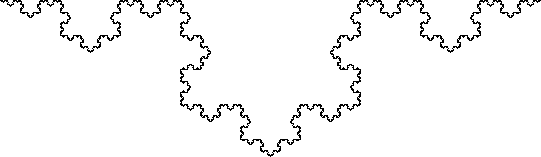
\includegraphics[width=\textwidth]{koch}
            \end{center}}
      \part Show that the length of the curve as $ n \to \infty $ becomes infinite.
      \part This curve is an example of a \textbf{continuous} curve that has \textbf{no tangent line anywhere}. Justify both bolded claims.
      \part Show that, if we start with an equilateral triangle and then add our equilateral triangles always on the outside, then the
            area enclosed by the final figure is precisely $ 8/5 $ of the original triangle area. The resulting figure, the Koch snowflake,
            is therefore a finite area bounded by a curve of infinite length.
    \end{parts}
\end{questions}

\clearpage
\section*{H-fractal: \texttt{hcurve.py}}
\lstinputlisting[language=Python]{fractals/hcurve.py}
\section*{Cantor set: \texttt{cantor.py}}
\lstinputlisting[language=Python]{fractals/cantor.py}

\clearpage
\section*{Sierpinski triangle: \texttt{sierp.py}}
\lstinputlisting[language=Python]{fractals/sierp.py}
\section*{Koch curve: \texttt{koch.py}}
\lstinputlisting[language=Python]{fractals/koch.py}


\end{document}
